\chapter{Related Work} \label{cpt-related-work}

\section{Voxel Scene Layout}

The voxel rendering in our evaluation relies on a volumetric representation of the scene.
It is particularly important that the voxel model not only includes the surface but also 
the space within the model. This constraint is often used in interactable use cases, where 
the model is split, cut or manipulated in any given way. [@TODO: Reference Minecraft] lets
the player take full control over the sandbox environment and allows adding or substracting 
any voxels. Essentially, the voxel data of every possible voxel within the playable space 
needs to be somehow present or encoded in memory, even though just a fraction of the voxels 
are actually drawn to the screen.\\

\subsection{Three Dimensional Grid} \label{subsec-three-dimensional-grid}

A basic approach for a scene representation is a three dimensional voxel grid. This 
approach relies on a fixed size grid where each grid cell represents one voxel.
To draw the voxels, a seperate buffer can hold additional voxel information, which 
can be accessed by a given grid cell index. The voxel data can store information about 
whether a voxel is present in that particular grid cell or not, which color the voxel 
should have, the normals for lighting calculation and any other data necessary.
This approach is relatively lightweight but inefficent for large grid sizes and low 
grid occupations. All grid cells need to be traversed to draw any given scene. This 
might include a lot of empty grid cells. Additionally, storing the voxel data seperately
introduces a pointer indirection on each step of the traversal, potentially leading to more 
cache misses.

\subsection{Octree Data Structure} \label{subsec-octree-data-structure}

[@TODO: source] proposes the use of a spatial container to optimize traversal. The use of an octree 
incorporates the relevant scene space and subdivides it into smaller child nodes. When inserting data 
into the octree, the position is evaluated and the data is being stored as a \emph{payload} in 
a node which includes the given position. If a node holds more payload instances than a specified threshold 
allows, it is split into eight child nodes and the payload originally present in the node is 
distributed onto the child nodes. This process is repeated until all data is finally inserted 
into the octree. The resulting octree maintains all the relevant payload data, having a deeper tree 
hierarchy where more data is present and a shallow hierarchy where almost no or no data is present.

[@TODO: Mention other spatial containers -> Binary Space Partitioning Trees]

Octrees like this can vary in their specific implementation, especially in how they maintain the 
payload. Some might store it right next to the octree node description, others might want to separate 
octree and payload data. Octree nodes could also be appended to a dedicated buffer and therefore be stored 
seperately to the tree hierarchy description. Such an approach would maintain chache coherency during an 
unordered traversal of all octree nodes. [@TODO: find appropriate sources]

When using hierarchical data structures dedicated vertex positions can be omitted and instead, 
the voxel position in space can be implicitly calculated from the hierarcical structure and the 
root nodes bounds. This allows for improvement of memory occupation, which is vital for loading and 
storing high resolution voxel scenes. A voxels state can be encoded into either visible (1) or empty (0).
A bitwise representation of voxels can significantly decrease the memory footprint which is a concept 
on which the next approach expand on.

\subsection{High Resolution Sparse Voxel Directed Acyclic Graphs} \label{subsec-highres-svo-dags}

\cite{Assarsson2013} use data redundancy to further generalize and optimize high resolution \ac{SVO}s. In their 
implementation the octree data structure relies on bitmasks, to encode the existance of child nodes. This way, 
empty nodes are ignored and the information can be easily stored within one byte. This child node mask uniquely 
identifies the layout of the nodes below and can also be used to store the voxel occupation of the leaf nodes.
Next, they make use of the fact, that an octree nodes position is uniquely identifed by the path along the 
nodes from root to leaf node. Since voxels can be encoded as either being present or not, and non-present 
voxels can be ignored, the data can be significantly reduced in size. Furthermore, equal child node masks 
can simply be shared between different parent nodes instead of being duplicated. \cite{Assarsson2013} suggest 
a buttom-up approach to remove redundant nodes and replace whole sub-trees of the octree by pointing to one 
instance of the same pattern within the tree, which is shown in figure \ref{fig:sparse-voxel-dag-creation}. 
This optimization can be recursively done to each layer in the tree hierarchy, resulting in an optimized version 
of the data structure. The resulting structure is a more general hierarchical data structure, namely a \ac{DAG}.

\begin{figure}[h]
    \centering
    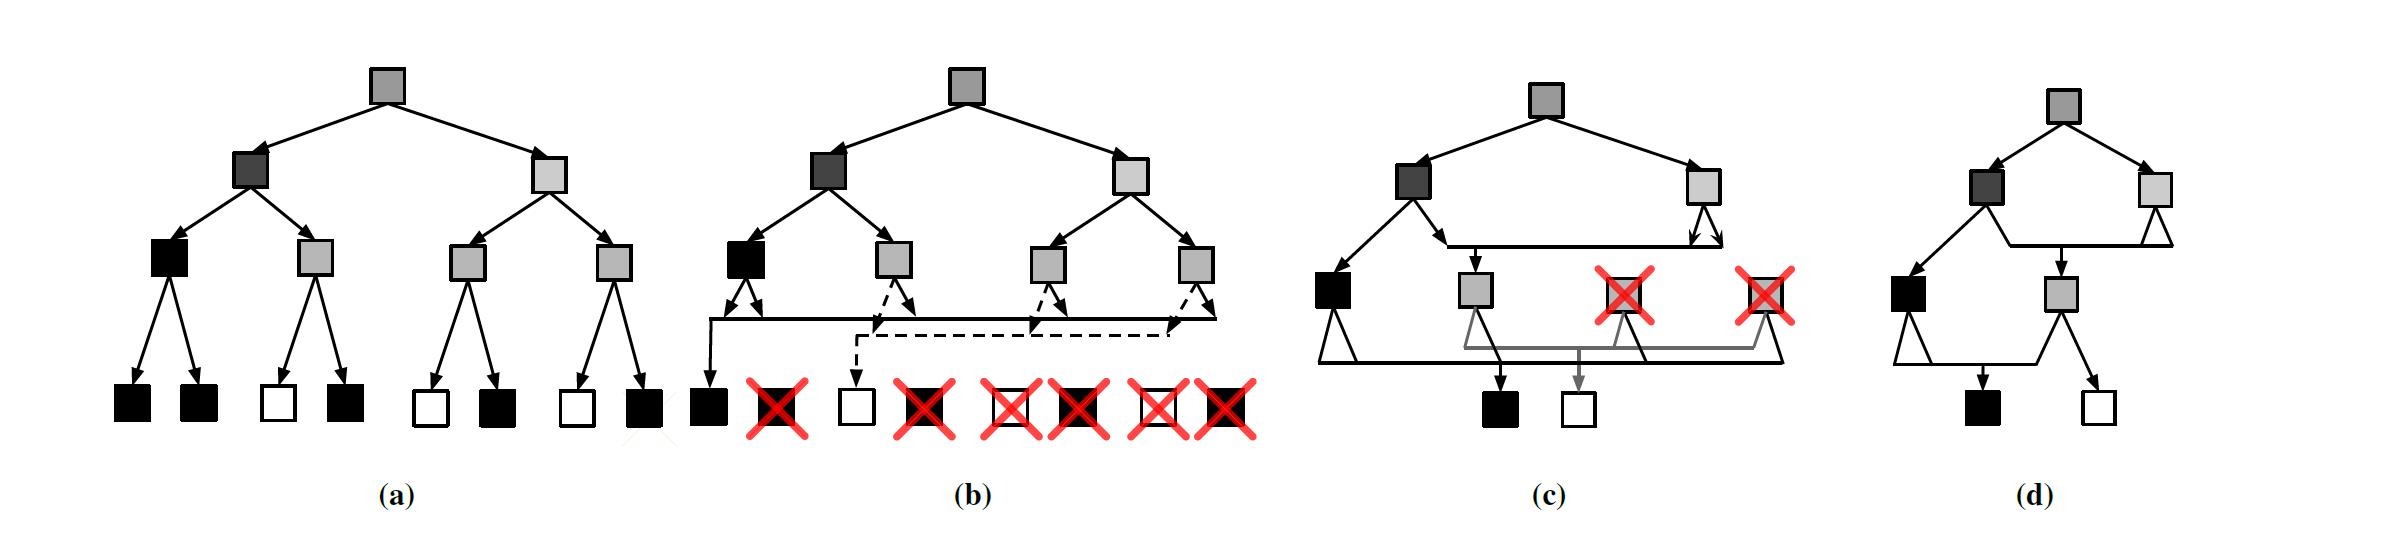
\includegraphics[width=\linewidth]{images/graphics/highres-sv-dag.png}
    \caption{Reducing a \ac{SVO} using the approach of \cite{Assarsson2013}.}
    \label{fig:sparse-voxel-dag-creation}
\end{figure}

This approach seems to be the best solution for reading, storing and optimizing octree data, although we use 
a more basic approach in our implementation. Nevertheless, this concept of optimizing voxel data is compatible 
with our use case and is highly recommended by us.

\section{Culling Techniques} \label{sec-culling-techniques}

\subsection{Backface Culling} \label{subsec-backface-culling}

\subsection{View Frustum Culling} \label{subsec-view-frustum-culling}

In combination with octree -> cull octree nodes 

\subsection{Point Based Occlusion Culling} \label{subsec-point-based-occlusion-culling}

\subsection{Hierarchical Z-Buffering} \label{subsec-hierarchical-z-buffering}

\subsection{Two-Pass Occlusion Culling} \label{subsec-two-pass-occlusion-culling}

\section{Mesh Shading}





% Wie strukturiere ich Related Work <-> Technical Background ? 
% Octrees haben keine bestimmte Quelle, daher eher technical background
% SV DAGs wiederum ist eher related work, auch wenn ich es nicht implementiere und es nicht wirklich 